\chapter{Theory}\todo{Lad det her med opdelingen simre.}
This thesis takes the perspective of viewing all eye information sources as well as their encodings as signals. This perspective is exceptionally useful when analysing uncertainty in a complex system composed of multiple information sources and with multiple goals. Additionally, it allows us to treat the objective of information obfuscation abstractly and thereby consider its use across multiple different applications. It turns out that any information extraction process can be defined in terms of just its ability to preserve the original information and be robust to noise. As a result, obfuscation methods are defined by competing goals of signal preservation for one information source (gaze) and signal degradation for another, e.g. the iris pattern. This chapter introduces and discusses the necessary prerequisites assuming a reader with knowledge of fundamental probability theory. The next chapter uses the presented theory to describe the abstract model and its implications.


%The proposed methodology and experiments rely on interpretations of eye tracking and iris recognition as communication systems of discrete signals. This requires a fundamental knowledge of information theory and signal processing which concern how uncertainty propagates and ...

%As presented in the overview, attributes such as gaze direction and personal identity can be represented as properties. These signals are encoded as physical properties which are transmitted through the medium of photons reflecting off of the eye onto a photosensitive camera sensor. This transmission creates an image, which is then processed further to ultimately decode the original properties. This is fundamentally similar to how a text message might be encoded and transmitted over a radio network to enable long distance communication.

%Information theory provides a number of tools for analysing such information transmission scenarios.
\section{Signals and information}
\begin{figure}
    \centering
    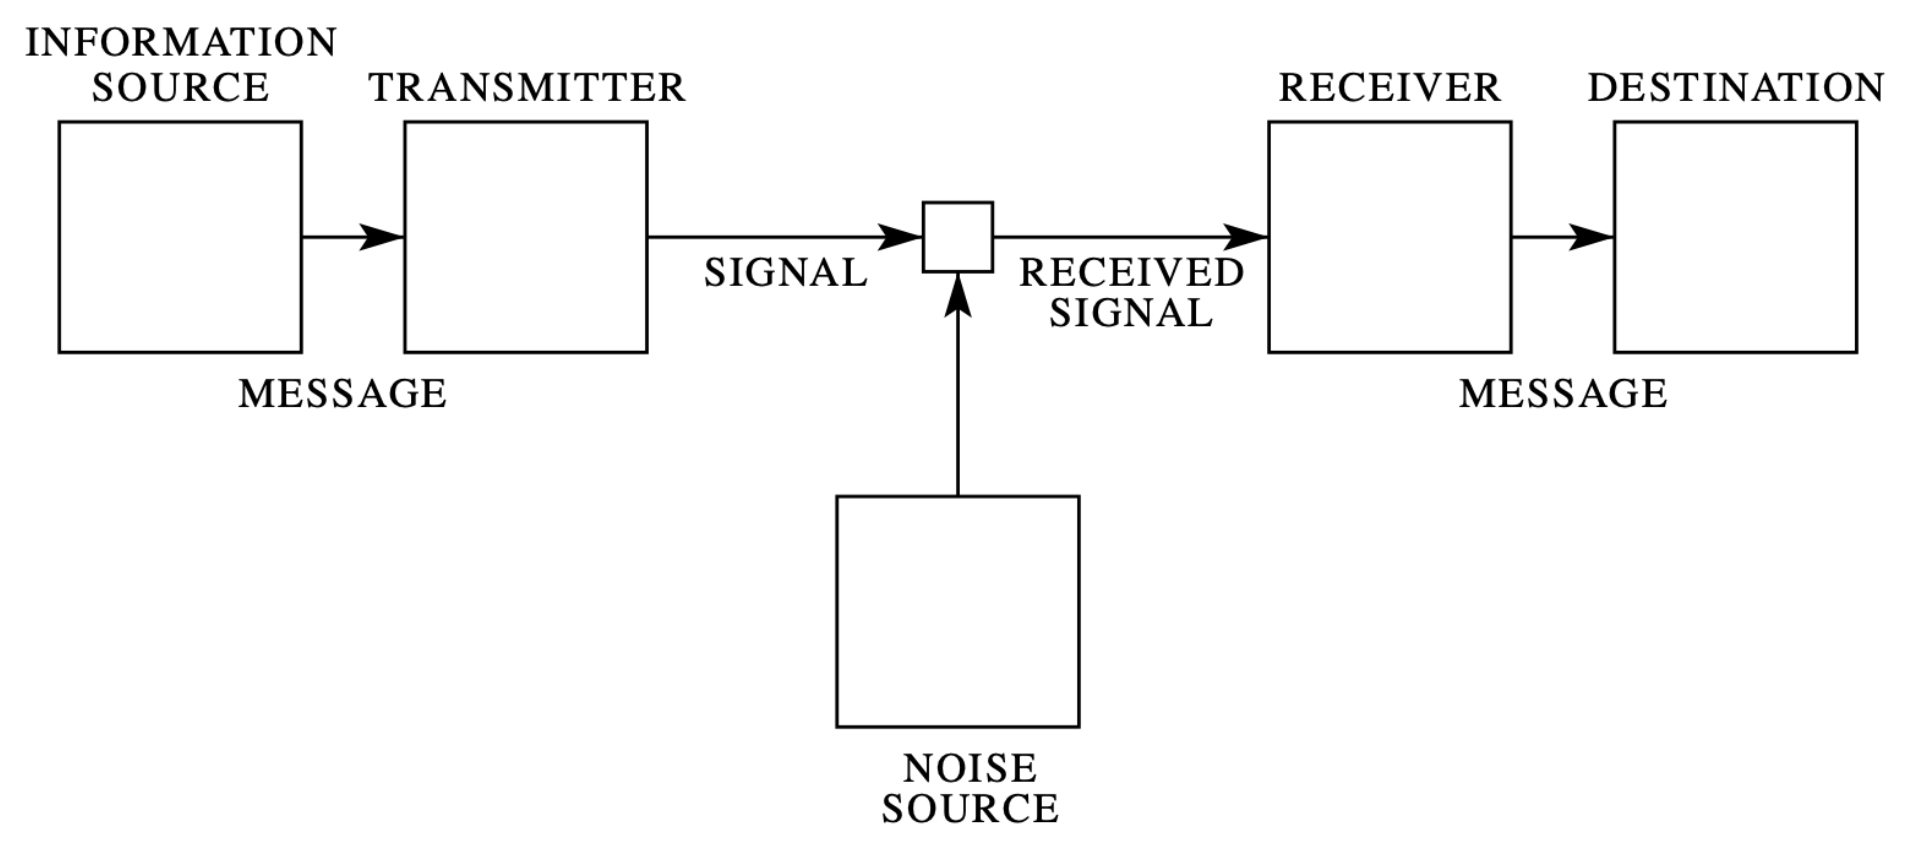
\includegraphics[width=0.8\textwidth]{figures/theory/comm-model.png}
    \caption{Diagram of communication system as depicted in \textit{A Mathematical Theory of Communication} \parencite{shannon1948mathematical}.}
    \label{fig:comm-model}
\end{figure}

\textit{Signal} is a rather vague term that is typically used to describe data that is transmitted over some medium and that contains \textit{meaningful information}. In this thesis, we use signal to denote any meaningful information that has been encoded by an arbitrary process. For example, the physical position and rotation of the eye is an encoding of several properties including point of regard. Only discrete signals are considered since images are the primary medium in eye tracking and they are discrete.\todo{Mangler lidt bindeled}

Information theory is a theoretical framework proposed by Claude Shannon for precisely measuring uncertainty in communication systems. As shown in \cref{fig:comm-model}, a communication system consists of an information source that is transmitted as a signal over a channel and then decoded back into its original representation. This basic diagram can be applied to many kinds of situations including error handling, compression, and, as proposed in this thesis, eye information obfuscation.


Information theory defines entropy as a measure of uncertainty. It is a logarithmic function of the randomness of the transmitted signal. 
The base measure is entropy, denoted $H$ which defines the optimal average encoding length of symbols $x_i$ drawn from a discrete distribution $X$ defined by
\todo{Alt herunder skal revideres med flere detaljer + mere historiefortælling}
\begin{definition}[Shannon entropy]
The Shannon entropy is the expectation of the self information $I(X)$ of each outcome of $X$:
\begin{equation}
    H(x) = \mathbb{E}[h_X(X)] = - \sum_i p_i\log p_i
\end{equation}
\end{definition}

with results in the units of bits. Different bases may be used for alternate units. A uniformly distributed discrete random variable has an entropy of $\log{N}$ which is maximal for its number of states. In terms of iris recognition, the entropy of code symbols (bits are typically used) can be used to calculate the expected amount of information present in the entire signal. For example, Daugman calculated the expected iris code entropy by fitting a binomial distribution to the iris code distance comparisons, which revealed an approximate 250 bits of information between codes (REF). This entropy only accounts for the information content in the final codes and thus does not account for noise added during the encoding and processing steps. 

\begin{definition}[Conditional entropy]
The Shannon entropy is the expectation of the self information $I(X)$ of each outcome of $X$:
\begin{equation}
    H(Y|X) = \sum_{x\in\mathcal{X}, y\in\mathcal{Y}} p(x, y)\log\frac{p(x, y)}{p(x)}
\end{equation}
\end{definition}

Mutual information is a measure that defines exactly how much entropy is preserved over a communications channel and is thus useful for determining how much information is actually captured by a specific process. Its definition is

\begin{definition}[Mutual information]
The Shannon entropy is the expectation of the self information $I(X)$ of each outcome of $X$:
\begin{equation}
    I(Y;X) = \sum_{x\in\mathcal{X}, y\in\mathcal{Y}} p(x, y)\log\frac{p(x, y)}{p(x)p(y)}
\end{equation}
\end{definition}

where $H(Y|X)$ is the conditional entropy which is a measure of the error added by the communication channel.

An extremely important property of signal entropy over a channel is that it can be decomposed into exactly the entropy carried over from the original signal (mutual information) and the noise introduced by the channel itself (conditional information) as shown visually in \cref{fig:comm-model}. This is encoded in the following relationship
\begin{align}\label{eq:entropy-law}
    H(X) = I(X;Y)+H(X|Y).
\end{align}
This is easily derived from the definitions of mutual information and conditional information
\begin{align*}
    I(X;Y)+H(X|Y) &= \sum_{x\in\mathcal{X}, y\in\mathcal{Y}} p(x, y)\log\frac{p(x,y)}{p(x)p(y)} + \left(-\sum_{x\in\mathcal{X}, y\in\mathcal{Y}} p(x, y)\log\frac{p(x,y)}{p(y)} \right) \\
    &= \sum_{x\in\mathcal{X}, y\in\mathcal{Y}} p(x,y)\left(\log{p(x,y)}-\log{p(x)}-\log{p(y)}-\log{p(x,y)}-\log{p(y)}\right)\\
    &= \sum_{x\in\mathcal{X}, y\in\mathcal{Y}} p(x,y)\log\frac{1}{p(x)}\\
    &= - \sum_{x\in\mathcal{X}} p(x)\log{p(x)}\\
    &= H(X).
\end{align*}

%For iris obfuscation, the goal is to minimise $I(R_{iris}, Q_{iris})$ and maximise $I(R_{gaze}, Q_{gaze})$. Measuring these directly is again not possible as the $Q$ signals are not the measured signals. The only known information source is the image $I$ where the two signals have been combined into a single signal. However, because $H(Q_{gaze})$ should be very low, i.e. it represents an encoding of just two real values, the mutual information between the original and obfuscated images $I(I, I^*)$ can be used as a proxy to measure the level of obfuscation. Additionally, for any set of signals $X, Y, Z$ where $Z = f_z(Y)$ and $Y= f_z(X)$, then $I(Z; Y) \leq I(Z;X)$ (REF to proof). Thus, it is an upper bound for the mutual information which makes the results much more useful.

Finally, the notion of channel capacity is used to define the maximum mutual information of a communications channel for any input distribution. It is defined as
\begin{align}
    C = \sup_{p(x)} I(X, Y).
\end{align}
The channel capacity of specific obfuscation methods define strong upper limits on the amount of information that is able to pass. If an obfuscation method has capacity below the minimum requirement for differentiation of a population given the optimal distribution (uniform), it is impossible to accurately differentiate between all individuals. In practice, however, the image signal which is measured contains orders of magnitude more information, making such guarantees unlikely, at least for the methods presented in this paper. Instead, we use the measure to evaluate the relative obfuscation of information.

\subsection{Properties of mutual information}
Mutual information can be generalised to multivariate cases. In ...

\begin{definition}
Given a set of $n$ random variables $X$, the mutual information between any subset $S\subset X$ is less than the mutual information of the whole set, i.e.
\begin{equation}
     I(S) \leq I(X)
\end{equation}
\end{definition}

proof: By the definition of measures, the mutual information $I$ is always non-negative, i.e. $I > 0$. Since $I(X) = I(X^1, \dots, X^{n-1}) - I(xxx)$, $I(X^1, \dots, X^{n-1}) \leq I(X)$.

% \section{Information theory}
% Uncertainty is similar to electrical voltage in that it represents a relative difference between knowledge and the lack thereof. Information is a measure of change in uncertainty over time. In other words, a highly uncertain message will impart the receiver with a large amount of information on arrival. If the receiver already knows part of the message, they will be less uncertain of its contents and therefore receive less information on arrival. 

% Information theory is a mathematical field which defines a useful theoretical model for information along with a large body of work In essence, information theory uses the language of probability and measures to define and quantify uncertainty of the signals and transmission procedures.



% Information represents the gap between not knowing and knowing and is thus inherently relative. It is similar to electrical voltage in that 

% The fact that information is a measure of uncertainty might seem counter intuitive when it feels like information should be the lack of uncertainty. This is, not surprisingly, the result of a misunderstanding. Information is not the randomness itself, but instead represents the amount of uncertainty removed when a random variable is observed.

% \begin{definition}[Self information]
% \begin{equation}
%     h_x(x) = -log(p_x(x))
% \end{equation}
% \end{definition}

% \begin{definition}[Shannon entropy]
% The Shannon entropy is the expectation of the self information $I(X)$ of each outcome of $X$:
% \begin{equation}
%     H(x) = \mathbb{E}[h_X(X)] = - \sum_i p_i\log p_i
% \end{equation}
% \end{definition}

% \begin{definition}[Joint entropy]
% The Shannon entropy is the expectation of the self information $I(X)$ of each outcome of $X$:\todo{Detailed description - shorten notation and provide explanations}
% \begin{multline}
%     H(X^1, \dots, X^n) = -\mathbb{E}[h_X(X^1, \dots, X^n)] =\\ - \sum_{x^1\in\mathcal{X^1}} \dots \sum_{x^n\in\mathcal{X^n}} p_{X^1, \dots, X^n}(x^1, \dots, x^n)\log p_{X^1, \dots, X^n}(x^1, \dots, x^n)
% \end{multline}
% \end{definition}

% \begin{definition}[Conditional entropy]
% The Shannon entropy is the expectation of the self information $I(X)$ of each outcome of $X$:
% \begin{equation}
%     H(Y|X) = \sum_{x\in\mathcal{X}, y\in\mathcal{Y}} p(x, y)\log\frac{p(x, y)}{p(x)}
% \end{equation}
% \end{definition}

% \begin{definition}[Mutual information]
% The Shannon entropy is the expectation of the self information $I(X)$ of each outcome of $X$:
% \begin{equation}
%     I(Y;X) = \sum_{x\in\mathcal{X}, y\in\mathcal{Y}} p(x, y)\log\frac{p(x, y)}{p(x)p(y)}
% \end{equation}
% \end{definition}

% \begin{equation}
%     H(X) = H(X|Y) + I(X;Y)
% \end{equation}

% \begin{definition}[KL divergence]
% The Shannon entropy is the expectation of the self information $I(X)$ of each outcome of $X$:
% \begin{equation}
%     D_{KL}(P||Q) = \sum_{x\in\mathcal{X}}p(x)\log\frac{p(x)}{q(x)}
% \end{equation}
% \end{definition}

% \begin{align}
%     I(Y; X) = D_{KL}(p_{x,y}||p_x\times p_y)
% \end{align}

% \chapter{Information and signals}
% This chapter reviews the theoretical tools used for the modelling and analysing eye information in this thesis. It is an expanded version of the presentation in the article and reveals more details of how the theoretical parts connect and have directly inspired the solution proposals.

\section{A model for eye information}
This section introduces a probabilistic model for understanding \emph{eye processing systems}. The purpose of the proposed model is to allow reinterpretation of gaze estimation, iris recognition, and potentially other eye information processes under a common reference frame. This makes it easier to understand how potentially conflicting goals such as iris obfuscation and gaze estimation interact and what trade-offs between them are likely to occur. Our hope is that the model will be used as a point of reference and comparison for future studies in this field.

An eye processing system is any software and/or hardware system which uses eye image capture to extract information about its subjects. It therefore covers both gaze estimation and iris recognition. 


%This allows analysis of how different goals affect each other. In the context of this paper, it specifically provides a framework for understanding how 

%This section presents a model and a methodology for understanding eye information processes. 
%This section presents an overview of the model used throughout the paper to examine the processes of iris recognition and gaze estimation from a common frame of reference. This allows critical analysis 





%This section presents a model for understanding how information flows through such systems and how image manipulations affect the information measurement processes. This allows us to evaluate and compare the obfuscation methods from a purely theoretical perspective which ... \todo{Overvej integration.. hvad giver det her? }

Any eye processing system has the goal of accurately measuring some properties of the real world through capture of eye images. These properties are encoded through physical processes as signals which are transformed and processed with the goal of isolating the property of interest from everything else. The systems therefore essentially have the function of signal denoising, albeit rather aggressively because anything but the target property is considered noise. Similarly, eye processing systems comprise a communication channel pipeline, with each physical encoding, image capturing, or transformation process forming a component in the pipeline. We propose a probabilistic graphical model which allows interpretations from both perspectives. 

%Similarly, information theory lets us define image processing as a communication system and analyse how uncertainty propagates and is added from noise. This lets us evaluate the effect of obfuscation methods directly on the image data. Although this is not in itself enough to demonstrate the effectiveness of the proposed methods, it creates a reference frame that does not depend on specific implementations of any algorithms. We propose a model which allows useful interpretations from both points of view and which has a simple graphical representation (shown in \autoref{fig:model}).

\begin{figure}
    \centering
    \begin{tikzpicture}[node distance=1.3cm]
        \node (q1) [] {$Q_1$};
        \node (qd) [right of=q1] {$\dots$};
        \node (qn) [right of=qd] {$Q_n$};
        \node (t1) [align=right, left of=q1] {(1)};
        
        %\node (e1) [rect, below of=q1] {$f_e^{(1)}$};
        %\node (ed) [right of=e1] {$\dots$};
        %\node (en) [rect, right of=ed] {$f_e^{(n)}$};
        %\node (t2) [align=right, left of=e1] {(2)};
        
        
        %\draw [arrow] (q1) -- (e1);
        %\draw [arrow] (qn) -- (en);
        
        \node (c) [rect, below of=qd] {$f_e$};
        \node (t3) [align=right, below of=t1] {(3)};
        \draw [arrow] (q1) -- (c);
        \draw [arrow] (qn) -- (c);
        
        \node (f1) [rect, below of=c] {$f_p$};
        \node (fd) [below of=f1] {$\dots$};
        \node (fn) [rect, below of=fd] {$f_n$};
        \draw [arrow] (c) -- node[anchor=east] {I} (f1);
        \draw [arrow] (f1) -- (fd);
        \draw [arrow] (fd) -- (fn);
        
        \node (t4) [align=right, below of=t3] {(4)};
        
        \node (dd) [below of=fn] {$\dots$};
        \node (d1) [rect, left of=dd] {$f_d^{(1)}$};
        \node (dn) [rect, right of=dd] {$f_d^{(n)}$};
        \node (t5) [align=right, left of= d1] {(5)};
        
        \draw [arrow] (fn) -- node[anchor=south east] {$I^*$} (d1);
        \draw [arrow] (fn) -- node[anchor=south west] {$I^*$} (dn);
        
        \node (r1) [below of=d1] {$R_1$};
        \node (rd) [right of=r1] {$\dots$};
        \node (rn) [right of=rd] {$R_n$};
        
        \draw [arrow] (d1) -- (r1);
        \draw [arrow] (dn) -- (rn);
    \end{tikzpicture}
    
    \caption{Eye information processing model: (1) Input properties. (2) Functions that encode the physical manifestation and uncertainties of the source properties. (3) Image capturing process. (4) Image processing steps which may typically be described as a single function. (5) Decoding functions that aim to extract original properties, e.g. an iris pattern or gaze direction.}
    \label{fig:model}
\end{figure}


%We define a model that allows easy analysis from both a signal-processing centric and probability centric view. 

Let an eye information processing system be defined by $\Lambda = \{Q, R, f_e, \mathcal{D}, \mathcal{P}\}$, where $Q=\{Q_1, \dots, Q_n\}$ is a set of source properties, $R=\{R_1,\dots,R_n\}$ is a set of output properties, $f_e$ is an encoding function, $\mathcal{D}=\{f_d^{(1)}, \dots, f_d^{(n)}\}$ is a set of decoding functions, and $\mathcal{P}=\{f_p^{(1)}, \dots, f_p^{(n)}\}$ is a set of processing functions. A graphical representation is shown in \autoref{fig:model}. The encoding functions in $f_e$ represent how properties are manifested as physical quantities and captured by a camera. This simplification retains the modelling of uncertainty in both processes. The results are given as $R_i = (f_d^{(i)}\circ f_p)(\hat{Q})$. To encode noise and information loss, all properties and functions are viewed as discrete signals composed of random samples of some distribution. The terms signal and property are therefore used interchangeably throughout this text.


\section{Analysis}\todo{Introduktion / revider flow}
The goal of any eye processing system is exactly to maximise mutual information and minimise conditional information between the decoded and original signals. This will be shown for both gaze estimation and iris recognition in (SECTION REF). For iris obfuscation, the goals compete, i.e. $I(R^{gaze};Q^{gaze})$ and $H(R^{iris}|Q^{iris})$ should be maximised while $H(R^{gaze}|Q^{gaze})$ and $I(R^{iris}|Q^{iris})$ should be minimised. This is problematic because the signals are both encoded in $I$ which is the signal we have to modify. 

\begin{theorem}
    For random variables $R$, $Q$ where $R=f(Q)$, then $f$ is a deterministic function if and only if $H(R|Q)=0$.
\end{theorem}

\begin{proof}

\begin{align}\label{eq:pr}
\begin{aligned}
    H(R|Q) = 0 &=-\sum_{r\in\mathcal{R}, q\in\mathcal{Q}} P(r,q)\log\frac{P(r,q)}{P(q)}\\
    &= -\sum_{r\in\mathcal{R}, q\in\mathcal{Q}} P(r,q)\left(\log P(r,q) - \log P(q)\right)\\
    &= \sum_{r\in\mathcal{R}, q\in\mathcal{Q}} P(r, q)\left(\log \sum_{r\in\mathcal{R}} P(r, q) - \log P(r,q)\right)
\end{aligned}
\end{align}
\todo{Check this stuff. Could easily contain small mistakes!}
By definition $\sum_{r\in\mathcal{R}} P(r, q) \geq P(r,q)$ and therefore each term must be non-negative. For any $P(r,q) > 0$ then, by \cref{eq:pr}, $P(q) - \log P(r,q) = 0$ and hence $P(q) = P(r,q)$. Consequently, only one value of $r$ can be positive, i.e. $P(r|q) = 1 \vee P(r|q) = 0$. In other words, $R$ is a deterministic function of $Q$ when the conditional information is $0$. 
\end{proof}

Maximising information involves the same problem in the opposite direction. Since $I(R;Q) = I(Q; R) = H(Q) - H(Q|R) = H(R) - H(R|Q)$, $I$ is maximal when both $H(Q|R)=H(R|Q)=0$ and hence, $I(Q;R)=H(R)=H(Q)$ and the function describing the system is deterministic and bijective. This is extremely important as it defines precisely the optimal solution to any eye processing system as the one that deterministically maps one distinct input to one distinct output.

\paragraph{Iris recognition}
Using the definition of an eye information system, iris recognition can be defined as the task of determining the probability of two iris codes $R^a$ and $R^b$ originating from the same source signals $Q^a = Q^b$ or different source signals $Q^a\neq Q^b$. Iris code is here used as a general term to cover any signal used for iris comparison. The probabilities are defined as $P(Q^a\neq Q^b|R^a, R^b)$, $P(Q^a\neq Q^b|R^a, R^b)$ and are determined by the comparison algorithm used. These are typically inferred by creating a distance metric $S = h(R^a, R^b)$ which is used for estimating the proxy distributions $P(S|Q^a\neq Q^b)$ or $P(S|Q^a\neq Q^b)$. In the most traditional case, iris recognition acceptance is performed by failing a statistical test of significance, i.e. determining that $P(S|Q^a\neq Q^b)$ is extremely unlikely. This was first proposed by Daugman (REF) and can be reformulated as
\begin{align}
\begin{aligned}
    h_0: & \quad s = h(R^a, R^b) &&\sim  P_{S|\hat{Q}^a\neq \hat{Q}^b}\\
    h_1: & \quad s && \sim  P_{S|\hat{Q}^a = \hat{Q}^b}.
\end{aligned}
\end{align}

In terms of the proposed eye information model, these distributions depend only on the internal system noise. 

We assume the original iris distribution to be uniform, i.e $P(Q)=1/N$ where $N$ is the total population. Given zero noise, $H(R|Q)=0$ and $H(R)=H(Q)$, $P(R)$ must be uniform on its support. As a result, $S$ which is defined to be $0$ when $R^a = R^b$, must have $P(S=0|Q^a = Q^b)=1$ and $P(S>0|Q^a \neq Q^b)=1$ since the original signals completely determine $S$. 

Because $S$ is bounded (here assumed to be normalised), an increase in noise $H(R|Q)$ increases the variance of $S$. Formally, as the noise approaches the maximum entropy of $R$, given by $M$, the distribution of $P(S)$ is
\begin{align}
\lim_{H(R|Q)\rightarrow M} P(S) = U(0, 1),
\end{align}
where $U(0, 1)$ denotes a discrete distribution of $M$ possible outcomes normalised to values in the $]0, 1[$ range. In the opposite direction, information may be lost due to low resolution image capture or bad decoding methods. This is represented by $I(R;Q)$. The relation in \autoref{eq:entropy-law} shows that mutual information limits the amount of information transmitted through the system. The limit is
\begin{align}
\lim_{I(R;Q)\rightarrow 0} P(S) = 0.
\end{align}

In other words, iris recognition systems are limited by their ability to transmit the iris pattern without introducing noise or capturing too little detail.

\paragraph{Gaze estimation}
%Gaze is defined as either the direction or point of visual attention of a given subject. This property is by definition at least partially subjective, as the point of attention does not always coincide with the fovea, but instead is at least partially controllable by the subject (REF). The physical encoding of gaze is then, at least when only observing the eye's immediate position and orientation, inherently probabilistic. This is captured by the model as the distribution $P(\hat{Q}|Q_{gaze})$, if the encoding function is split between physical encoding and image capture such that $I=f_{capture}(\hat{Q})$ and $\hat{Q}=f_{physical}(Q_{gaze}, \dots)$. 

%Each additional step in a given gaze estimation system introduces some amount of additional noise given by its imperfections. Robust gaze estimation can therefore be defined as transformations and decoders that have low noise-rates for large variations in signal distributions. Consequently, a non-robust system is characterised by having low noise-rates only for a narrow subset of input signals. 

The definition of an ideal gaze estimation system is one that minimises the conditional information $H(R^{gaze}|Q^{gaze})$ while maximising the entropy $H(R^{gaze})$. Since $Q^{gaze}$ represents only the distribution of a single gaze signal, we may add that the capacity of $f^{gaze}_d \circ f_p^{(n)} \circ \dots \circ f_p^{(1)} \circ f_e$ should have $\mathcal{C} = \max H(R^{gaze})$, i.e. the capacity should be equal to the maximum entropy of a specific gaze point. For example, if the gaze is described as two $16$-bit integers, the capacity should be $32$ bits.

This goal is reflected by the typical least squares approach to optimising the gaze decoder function $f^{gaze}_d$. In the notation of an eye processing model, gaze function optimisation is typically expressed
\begin{align}
    \min \mathbb{E}_{q}\left[\norm{\hat{Q}^{gaze} - \left(f^{gaze}_d \circ f_p^{(n)} \circ \dots \circ f_p^{(1)} \circ f_e\right)(Q^{gaze})}_2\right],
\end{align}
where $\hat{Q}^{gaze}$ is an approximation of $Q^{gaze}$ based on the assumption that the subject looked at a known fixed point at a certain point in time.



